\appendix

\section{Software Repositories} \label{apx:software-repos}

\subsection{Communication Protocol Specifications} \label{apx:comm-spec-repos}

The protocol used for transmitting telemetry data from the rocket to the ground station can be found in the
\href{https://github.com/CarletonURocketry/telemetry-format/blob/gh-pages/radio_packet_format.pdf}{CarletonURocketry
    telemetry-format repository.}

The protocol used for communication between nodes on the hybrid control system network can be found in the
\href{https://github.com/CarletonURocketry/hybrid-comm-format/blob/gh-pages/spec.pdf}{CarletonURocketry
    hybrid-comm-format} repository.

\subsection{Telemetry System Repositories} \label{apx:telem-repos}

All of the previous year's telemetry system code designed for the transmitter running QNX can be found here in the
\href{https://github.com/CarletonURocketry/qnx-stack}{qnx-stack} repository. All of the sub-processes making up the
telemetry system are listed there as GitHub sub-modules. You can also find the early design document LaTeX files for
last year's preliminary design review there. It is not up to date with the final design of the system when it launched.

The code for InSpace's ground station receiver can be found in the
\href{https://github.com/CarletonURocketry/ground-station}{CarletonURocketry ground-station} repository. This is the
code responsible for receiving incoming packets over LoRa and converting them into JSON for the ground station UI to
display.

The code for InSpace's ground station UI can be found in the
\href{https://github.com/CarletonURocketry/ground-station-ui}{CarletonURocketry ground-station-ui} repository. This is
the system responsible for displaying live telemetry data.

\subsection{Hybrid Control System Repositories} \label{apx:hybrid-control-repos}

The code for InSpace's hybrid control system UI can be found in the
\href{https://github.com/CarletonURocketry/hybrid-engine-ui}{CarletonURocktry hybrid-engine-ui} repository. This code
is responsible for displaying telemetry from the hybrid control system, such as pressure, temperature and mass measured
by the load cell.

The code for InSpace's hybrid control system can be found in the
\href{https://github.com/CarletonURocketry/hysim}{CarletonURocketry hysim} repository. This code simulates all three
types of nodes within the control system: the telemetry client, a control client and the launch pad control system
itself. The code is intended to run on any POSIX system with networking capabilities so that it's core logic can be
tested before being put on real control system hardware.

\section{littlefs} \label{apx:littlefs}

\textit{littlefs} is a power-failure safe file-system designed for embedded systems where data integrity is critical and
space is constrained. It is primarily used on small NOR and NAND flash memory banks, but also supports SD and eMMC. The
repository for \textit{littlefs} can be found on \href{https://github.com/littlefs-project/littlefs}{GitHub}, and you can read more about how it works in their
\href{https://github.com/littlefs-project/littlefs/blob/master/DESIGN.md}{design document}.

The NuttX documentation for \textit{littlefs} support can be found
\href{https://nuttx.apache.org/docs/latest/components/filesystem/littlefs.html}{here, on their website}.

\section{RN2483} \label{apx:rn483}

The RN2483 is a LoRa radio transceiver made by Microchip. Its datasheet can be found
\href{https://ww1.microchip.com/downloads/aemDocuments/documents/OTH/ProductDocuments/DataSheets/RN2483-Low-Power-Long-Range-LoRa-Technology-Transceiver-Module-DS50002346F.pdf}{here},
and the command options for controlling the radio can be found
\href{https://ww1.microchip.com/downloads/en/DeviceDoc/RN2483-LoRa-Technology-Module-Command-Reference-User-Guide-DS40001784G.pdf}{here}.

\section{PCB Schematics} \label{apx:pcb-schematics}
\subsection{MCU Board Schematics}
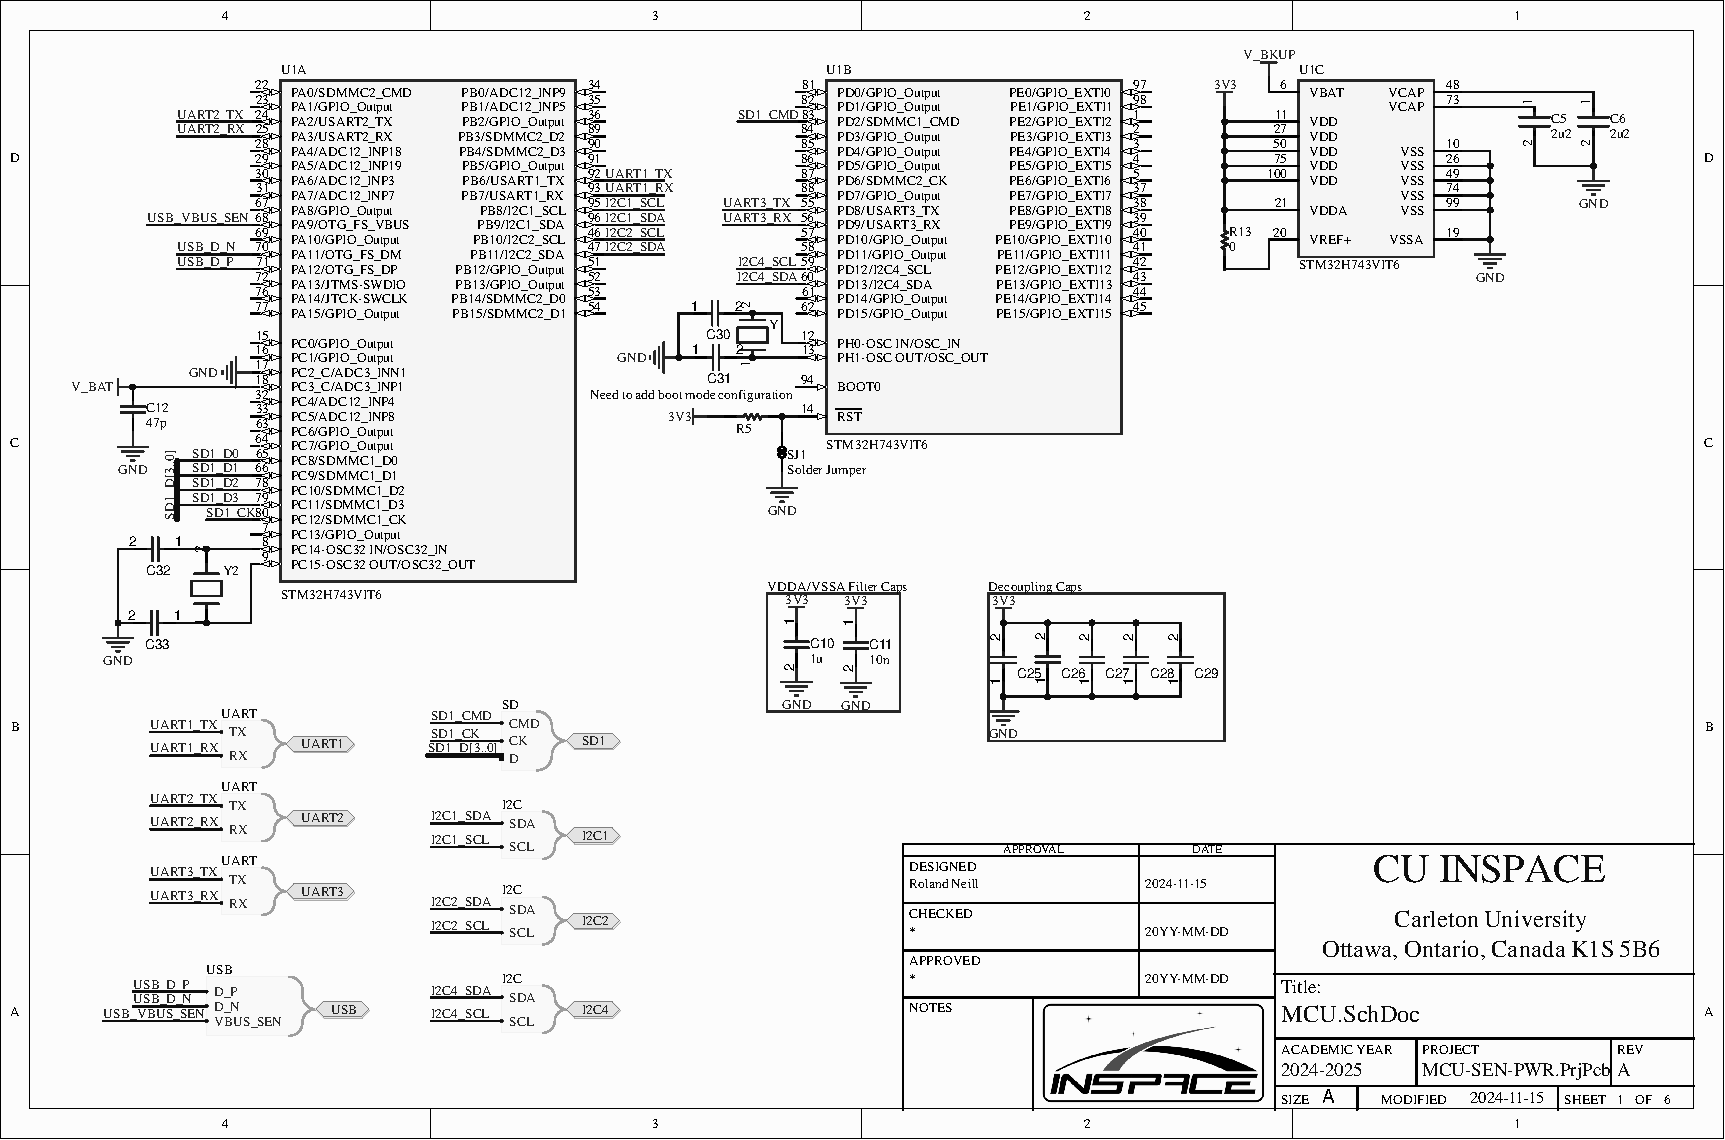
\includepdf[pages=-, angle=90]{assets/schematics/mcuBRD.pdf}

\subsection{Radio Board Schematics}
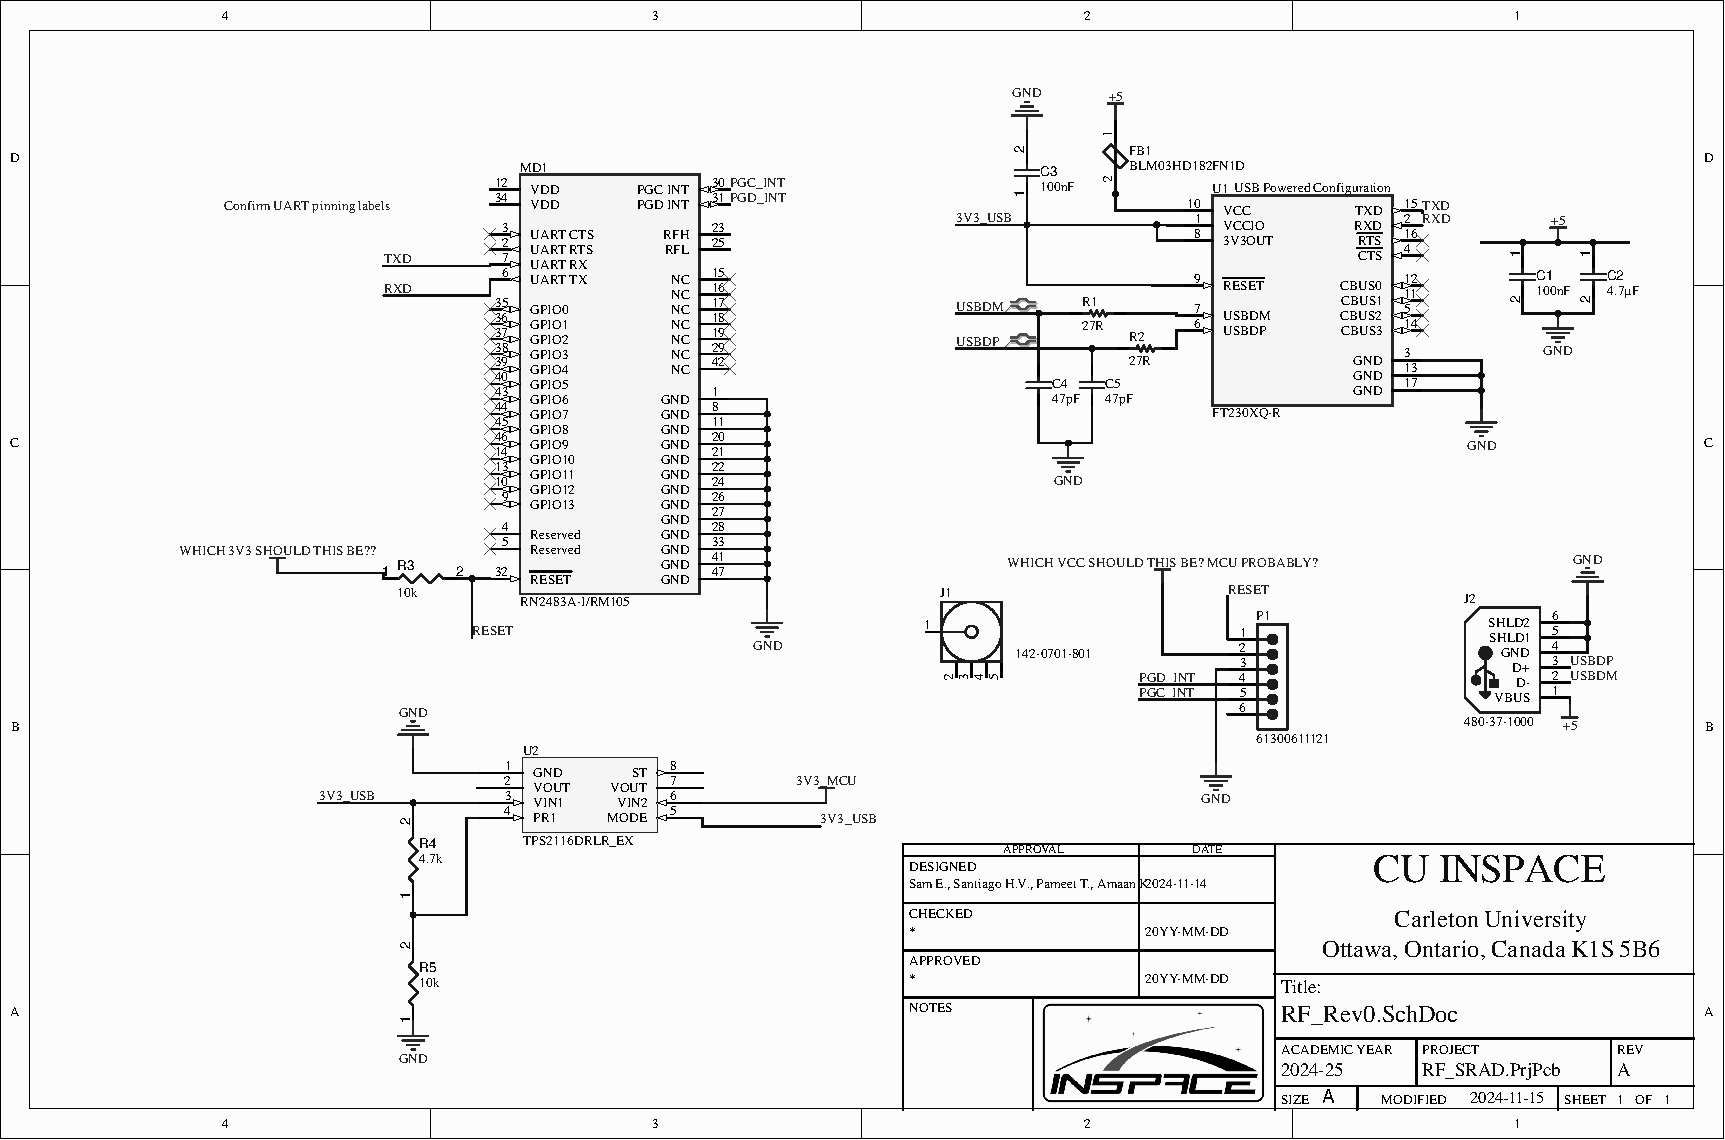
\includepdf[pages=-, angle=90]{assets/schematics/radioBRD.pdf}